\documentclass{article}
\usepackage{listings, xcolor, graphicx, inconsolata}
\setlength{\parindent}{0pt}

\definecolor{lgray}{rgb}{0.95, 0.95, 0.95}
\definecolor{lgray2}{rgb}{0.75, 0.75, 0.75}

\lstset{
  language=C++,
  aboveskip=10pt,
  belowskip=10pt,
  frame=leftline,
  xleftmargin=15pt,
  framexleftmargin=20pt,
  breaklines=true,
  basicstyle=\small,
  showstringspaces=false,
  backgroundcolor=\color{lgray},
  rulecolor=\color{lgray2},
  basicstyle=\ttfamily\footnotesize,
  keywordstyle=\color{blue},
  stringstyle=\color{red},
  commentstyle=\color{green},
  numbers=left,               
  numberstyle=\tiny\color{gray},
  stepnumber=1
}

\title{CS135; User-Defined Functions}
\author{Gael Zarco}
\date{\today}

\begin{document}

\maketitle

Functions are often called \textbf{modules} in C++.

% SECTION 1 %
\section{Pre-Defined Functions}
Examples of pre-defined functions include (each are of type \texttt{double}):
\begin{itemize}
  \item \texttt{pow(x, y)} calculates $x^y$.
  \item \texttt{sqrt(x)} calculates nonnegative square root of $x$ for $x >= 0$.
  \item \texttt{floor(x)} calculates the largest whole number that is $<=x$.
\end{itemize}
The $x$ and $y$ values in these functions are called \textbf{parameters} or
\textbf{arguments}. A function's type is that of the returned value.

\vspace{8pt}
More Function Examples:
\begin{center}
    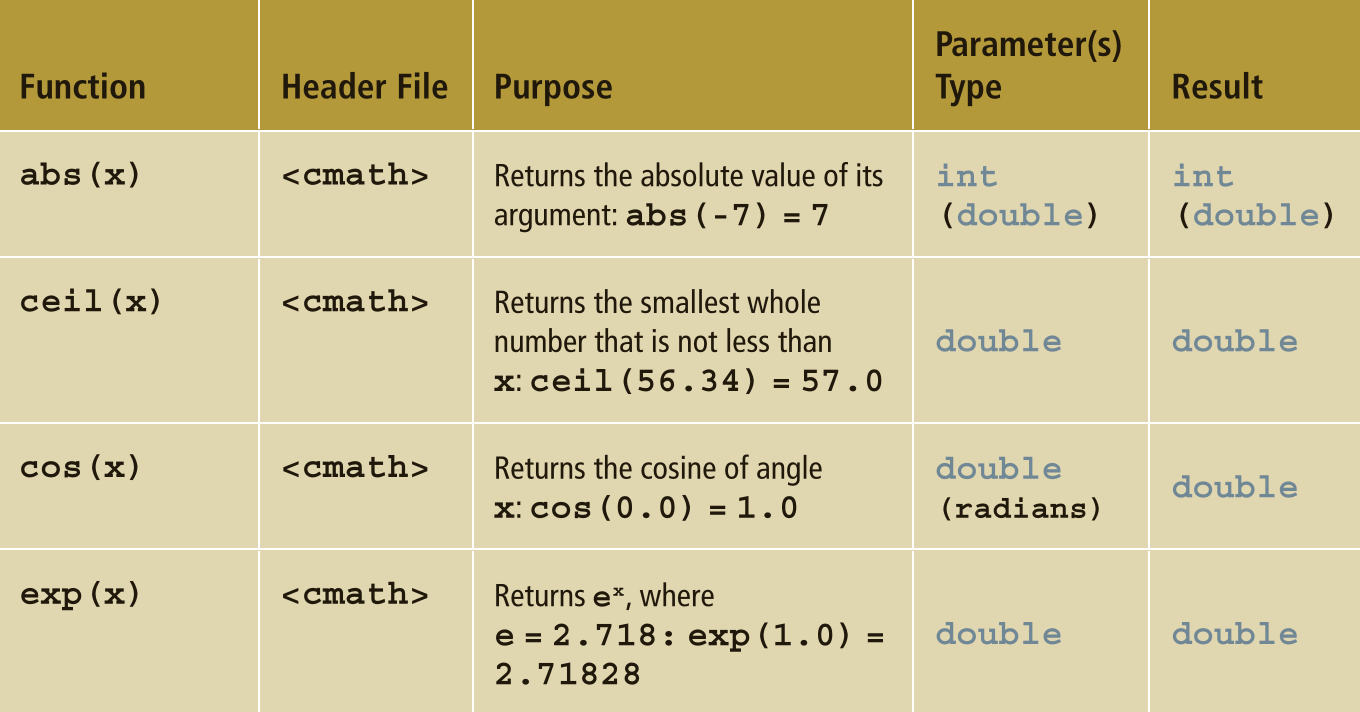
\includegraphics[width=0.9\textwidth]{pre-def-func-1.png}
    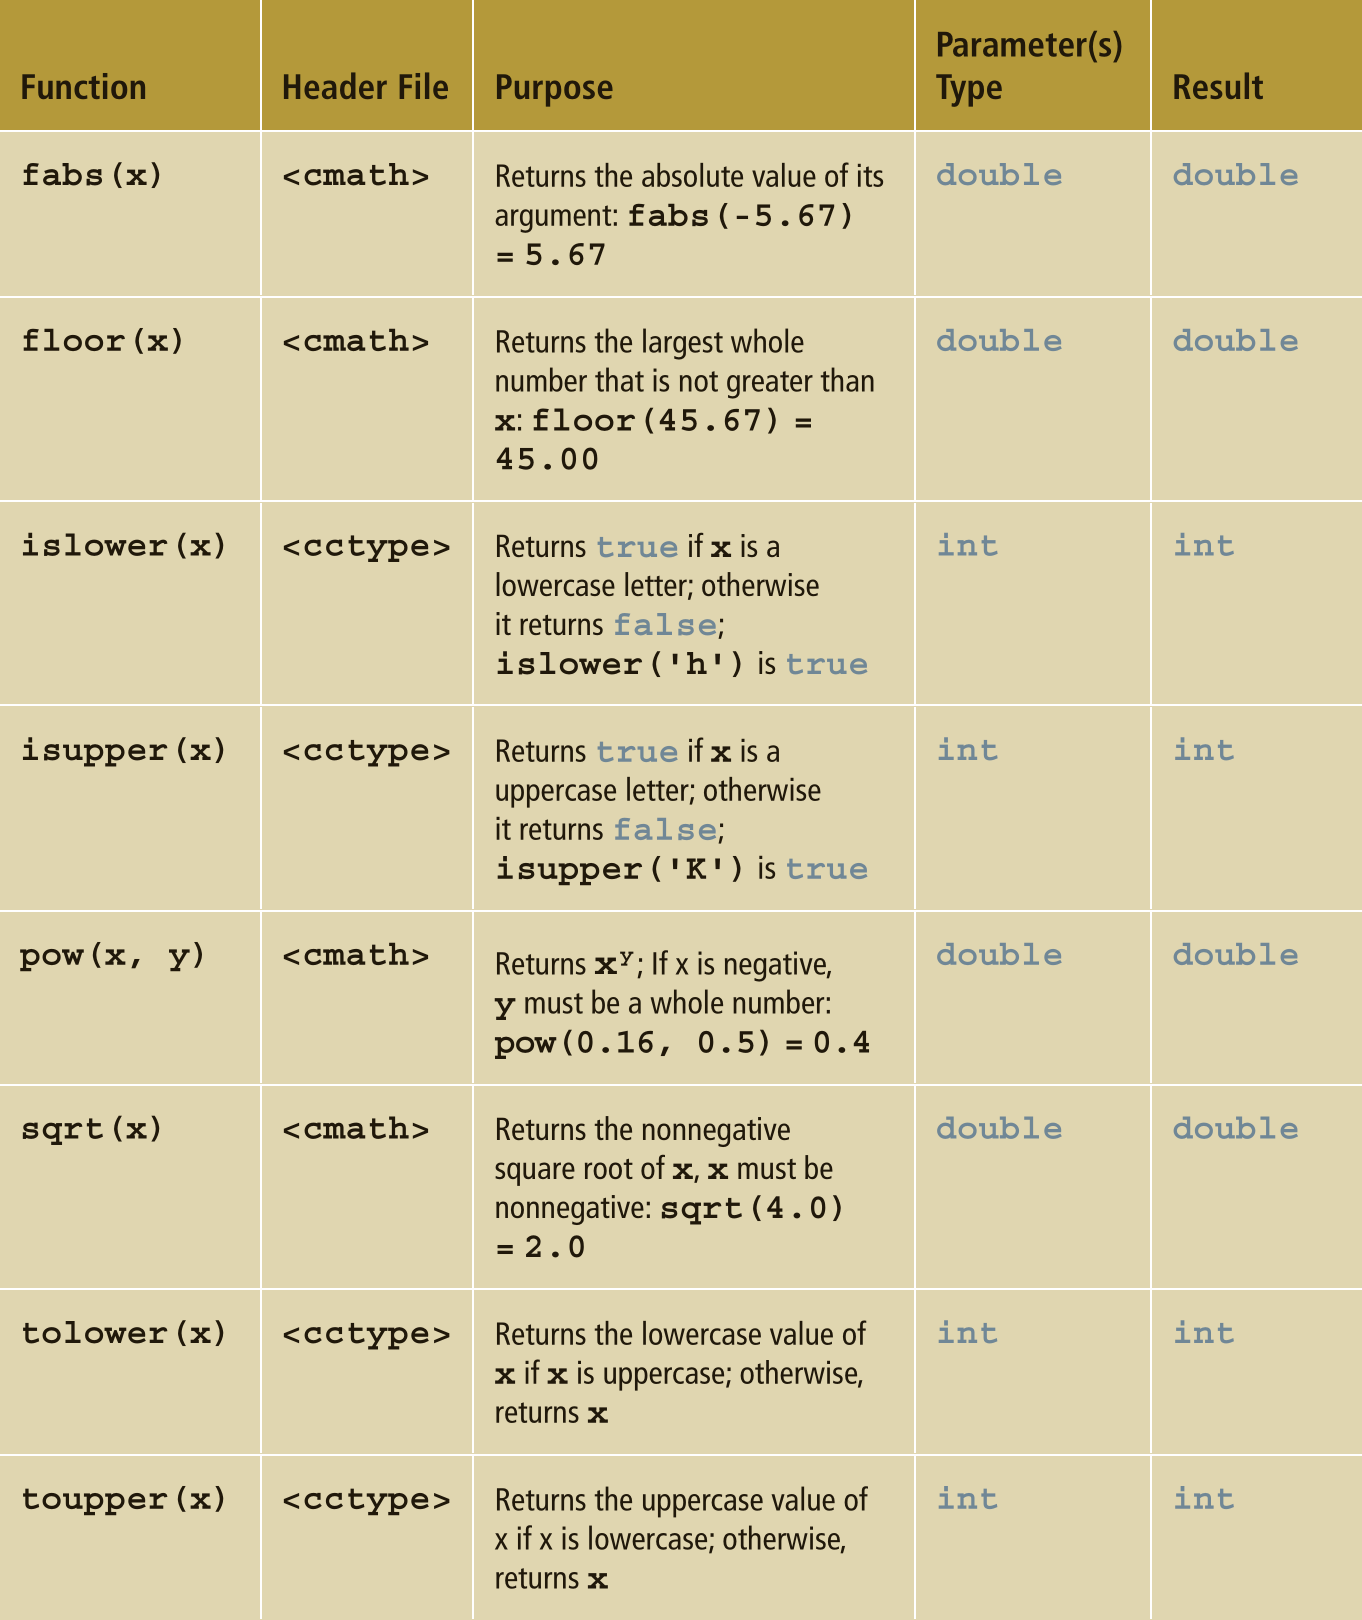
\includegraphics[width=0.9\textwidth]{pre-def-func-2.png}
\end{center}

% SECTION 2 %
\section{User-Defined Functions}
User-defined functions in C++ are classified into two categories:
\begin{itemize}
  \item \textbf{Value-Returning Functions} use \texttt{return} statement to
    return a value (has a data type).
  \item \textbf{Void-Returning Functions} do not have a return type; do not use
    \texttt{return} statement.
\end{itemize}

% SECTION 2-1 %
\subsection{Value-Returning Functions}
C++ functions such as pow, abs, islower, and toupper are examples of
value-returning functions. Use these functions by including the \textit{header file} in
your program and knowing the following:
\begin{enumerate}
  \item The name of the function.
  \item The \textit{parameters} (if applicable)
  \item The data type of each parameter.
  \item The type of the function
  \item The code required to accomplish the task (both value-returning and void).
\end{enumerate}

To elaborate on \textit{5}, the \texttt{abs} function may have the following
definition:
\begin{lstlisting}[caption={\texttt{abs} Function}]
int abs(int number) {
  if (number < 0)
    number = -number;

  return number;
}
\end{lstlisting}

The function declared in the heading of the \texttt{abs} function defintion is
known as the \textbf{Formal Parameter} (\texttt{number}). The heading within a 
function definition defines all formal parameters.

\vspace{8pt}
The \textbf{Actual Parameters} of a function are the variables passed into the
function and copied into the formal parameters.

\begin{itemize}
  \item \textbf{Formal Parameter}: A variable declared in the function heading.
  \item \textbf{Actual Parameter}: A variable or expression listed in a call to a function.
\end{itemize}

For example:
\begin{lstlisting}[caption={\texttt{pow} Function Header}]
  double pow(double base, double exponent)
\end{lstlisting}

\textit{In the code below, the values of \texttt{u} and \texttt{v} are copied into
\texttt{base} and \texttt{exponent}:}

\begin{lstlisting}[caption={\texttt{pow} Actual Parameter Example}]
  double u = 2.5;
  double v = 3.0;
  double x, y;

  x = pow(u, v);
  y = pow(2.0, 3.2) + 5.1;
  cout << u << " to the power of 7 = " << pow(u, 7) << endl;
\end{lstlisting}

\textit{The values of \texttt{2.5} and \texttt{3.5} are also copied into \texttt{base}
and \texttt{exponent}; as are \texttt{u} and \texttt{7}.}

\vspace{8pt}
A value-returning function can be used:
\begin{itemize}
  \item As an assignment statement.
  \item As a parameter in a function call.
  \item In an output statement.
\end{itemize}

Syntax Breakdown:
\begin{center}
    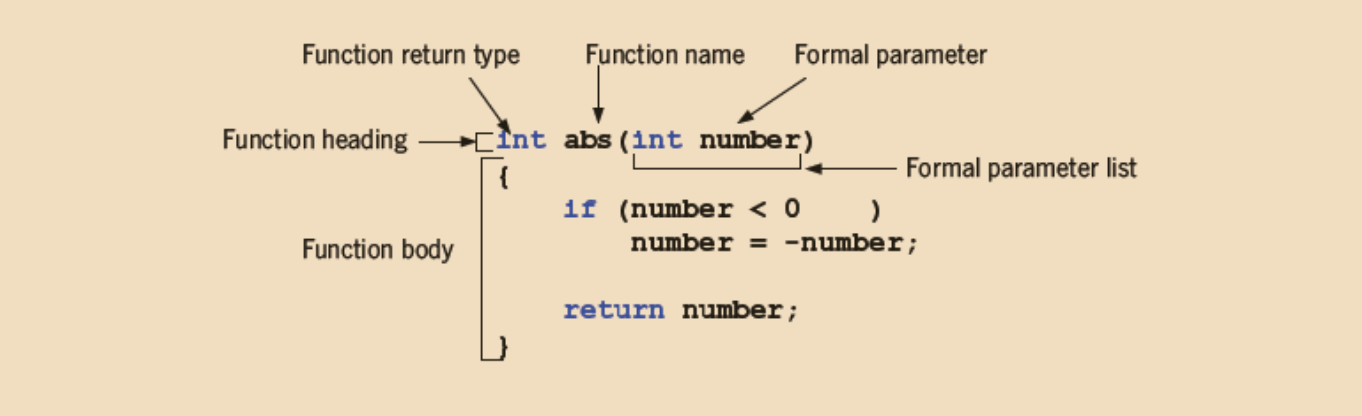
\includegraphics[width=0.9\textwidth]{val-ret-func-syntax.png}
\end{center}
 
\subsection{Formal Parameter List}
\begin{lstlisting}[caption={Formal Parameter List Syntax}]
dataType identifier, dataType, identifier...
\end{lstlisting}

\subsection{Function Call}
\begin{lstlisting}[caption={Value-Returning Function Syntax \& Example}]
functionName(actual parameter list)

// Example
x = abs (-5);
\end{lstlisting}

\subsection{Actual Parameter List Syntax}
\begin{lstlisting}[caption={Syntax For Actual Parameter List}]
expression or variable, expression or variable
\end{lstlisting}

A function's formal parameter list may be empty, however parentheses are still
needed.
\begin{lstlisting}[caption={Empty Formal Parameter List Function Call}]
functionType functionName()
\end{lstlisting}

A value-returning function is also called an expression. Calling a function
causes the function body to execute.

\vspace{8pt}
Function calls can be:
\begin{itemize}
  \item part of an assignment or output statement.
  \item parameter in a function call.
\end{itemize}

\subsection{\texttt{return} Statement}
Functions return values using a \texttt{return} statement; passes the values
outside the functions scope.

\begin{lstlisting}[caption={\texttt{return} Statement Syntax}]
return expr;
\end{lstlisting}

\texttt{expr} is a variable, constant value, or expression. \texttt{expr} is
evaluated and its value is returned.
\begin{itemize}
  \item The data type must match function type.
\end{itemize}

When a \texttt{return} statement executes in a function:
\begin{itemize}
  \item The function is immediately terminated.
  \item Function call statement is replaced by the value of the \texttt{return}
    statement.
  \item Terminates the program if called within the \texttt{main} function.
\end{itemize}

\begin{lstlisting}[caption={Example program using \texttt{return}}]
double larger(double x, double y) {
  double max;

  if (x >= y)
    max = x;
  else
    max = y;

  return max;
}
\end{lstlisting}

The variable \texttt{max} is called a \textbf{Local Variable Declaration}, in
which \texttt{max} is a variable local to the function \texttt{larger}.

\vspace{8pt}
Syntax breakdown:
\begin{center}
    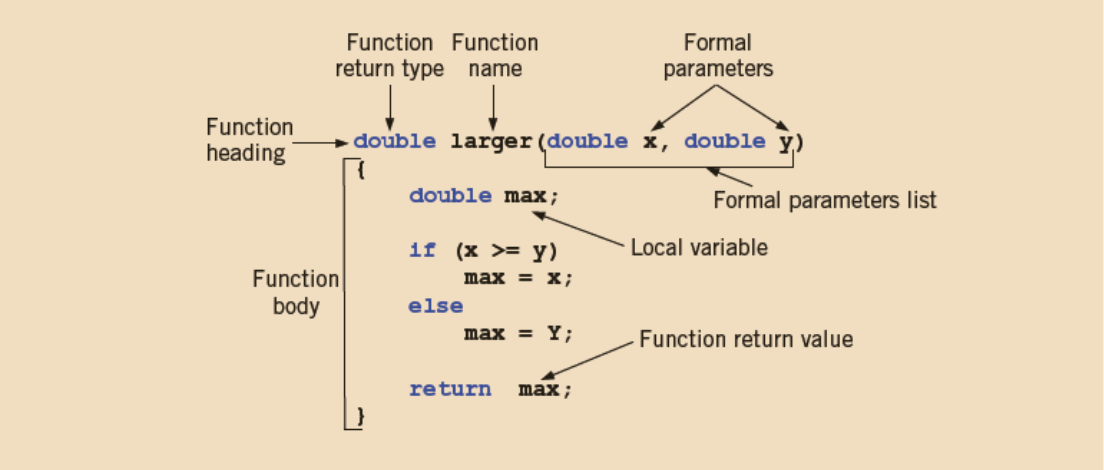
\includegraphics[width=0.9\textwidth]{larger-ret-func-ex.png}
\end{center}

\subsection{Function Prototype}
To work around the problem of undeclared identifiers regarding where to place
function definitions in a program, place \textbf{Function Prototypes} before
function definitions including \texttt{main}.
\begin{itemize}
  \item Function prototype is \textit{not} a definition.
  \item Gives the program the name of the function, number and data types of
    parameters, and data type of returned values.
  \item It is just enough information to let C++ use the function.
  \item Serves as a promise that the full definition will appear elsewhere in
    the program (will compile but \textit{not} execute if missing defintion).
\end{itemize}

The \textbf{Function Prototype} is a function heading, terminated by a
semicolon, \texttt{;}, without the function body.

\begin{lstlisting}[caption={Function Prototype Syntax}]
functionType functionName(parameter list); \end{lstlisting}

\section{Flow of Execution \& Compilation}
Execution always begins at the first statement in the \texttt{main} function.
\begin{itemize}
  \item Other functions executed only when called.
  \item Function prototypes appear before any function definition (translated by
    compiler first).
  \item Function call transfers control to the first statement in the body of
    the called function.
  \item End of called function returns control to the point immediately before
    the function call (returned value replaces the function call statement).
\end{itemize}

% \section{Choosing the Correct Looping Structure}
% \begin{itemize}
%   \item If you know the number of repetitions needed $\rightarrow$ \texttt{for} loop.
%   \item If you do not know and it \textbf{could be 0} $\rightarrow$ \texttt{while} loop.
%   \item If you do not know and it is \textbf{at least 1} $\rightarrow$ \texttt{do...while} loop.
% \end{itemize}
% 
% \vspace{8pt}
% Differences between loops:
% \begin{itemize}
%   \item \texttt{do..while} and \texttt{while}: \texttt{expression}
%     is evaluated immediately after \texttt{continue} \allowbreak statement.
%   \item \texttt{for}: \texttt{update statement} is executed after
%     \texttt{continue} statement $\rightarrow$ \texttt{loop condition} executes.
% \end{itemize}
%
\end{document}
